
% SECTION : logistic_regression {{{
\section{Logistic Regression}
\label{sec:logistic_regression}
\parindent=0em

% 	SUB-SECTION : motivation {{{
\subsection{Motivation}
\label{ssec:motivation}
\parindent=0em

Logistic Regression is a classification algorithm. The objective of logistic
regression is to categorize unseen datapoints into one of multiple categories.
First we will deal with the simple case for explanation , where we only have to
categorize an input data point into one of two categories. Namely it has to be
either true / false , 1/0 , spam / not spam , malignant / benign etc \ldots
So we have :

\[ y \in \left\{ 0,1 \right\} \]

Where 0 is also known as the negative class (e.g. benign , not spam , false
\ldots) , and 1 is the positive class (e.g. malignant , spam , true \ldots).
Later we will deal with more than two classes so y will look like :

\[ y \in \left\{ 0,1,2,3, \ldots , n \right\} \]

The linear regression hypothesis is a good starting point but our hypothesis
\( h_{\theta} (x) \) can be any continuous value. \\

However we only want it predict binary values 0 or 1. We need to find a way to
restrict it to this range , i.e.  we want \( 0 \leq h_{\theta} (x) \leq 1 \) ,
where \( h_\theta (x) = \theta_0 + \theta_1 x \) or in vector notation : \(
	h_{\theta}(X) = \Theta^T X \). To achieve this goal we will be using the
logistic function ( also called the sigmoid ). Given by the equation : 

\[
	\begin{array}{ l@{} l@{} }
		g(x)
		& =
		\frac{1}
		{
			1+e^
			{
				\left( - x \right)
			}
		}
	\end{array}
\]

 % sigmoid  {{{

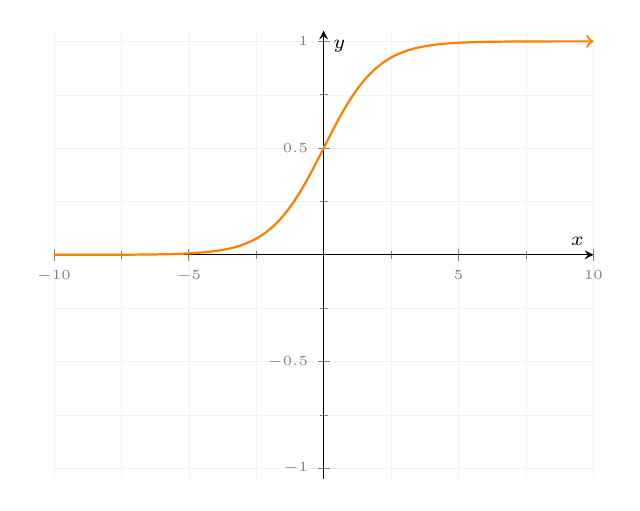
\begin{tikzpicture}
% axis settings {{{

\begin{axis}[
%	title          = graph_name,
	axis x line    = middle, % x-axis position
	axis y line    = middle, % y-axis position
	minor tick num = 1,      % num axis ticks
	grid           = both,
	grid style     =
	{
		line width=.1pt,
		draw=gray!10
	},
	xmax = 10,
	xmin = -10,
	ymax = 1.05, % 0.05 is to show the ->
	ymin = -1.05,
	tick label style = {
		font = \tiny,
		color = gray
	},
%	extra x ticks={3,1},
%	extra x tick labels={$\leftarrow$,$\rightarrow$},
%	extra y ticks={3,1},
%	extra y tick labels={$\leftarrow$,$\rightarrow$},
	legend style =
	{
		draw         = none, % remove legend bounding box
		font         = \tiny,
		legend pos   = outer north east,
		cells        = {anchor = west},
		fill         = gray,
		fill opacity = 0.4,
		text opacity = 1
	},
	xlabel       = {$\scriptstyle x$},
	ylabel       = {$\scriptstyle y$},
	xlabel style =
	{
		at     = {(ticklabel* cs:1)},
%		anchor = north west
	},
	ylabel style=
	{
		at     = {(ticklabel* cs:1)},
%		anchor = south west
	}
]
% }}}

\coordinate (O) at (0,0);

\addplot [
	domain=-10:10,
	no marks,
	samples=100,
	thick,
	orange,
	->
]
{1/(1+exp(-x)};
%\addlegendentry{$\frac{1}{1+e^{-x}}$};

\end{axis}
\end{tikzpicture}

% }}}

This is a function that will always output a value between 1 and 0 , i.e. , $ 0
\leq h_{\theta} (x) \leq 1 $. So we just take the output of our hypothesis
function , and pipe it through to the sigmoid in order to map it down to the
range we want. Which looks like :

\[
\begin{array}{ l@{} l@{} l@{} }
	h_\theta(x)
	& = g(\theta_0 + \theta_1 x) 
	& =
	\frac{1}
	{
		1+e^
		{
			-
			\left(
				\theta_0 + \theta_1 x
			\right)
		}
	}
	\\
	h_\theta(X)
	& = g(\Theta^T X)
	& =
	\frac{1}
	{
		1+e^
		{
			-
			\left(
				\Theta^T X
			\right)
		}
	}
	\\
\end{array}
\]

However $h_\theta(x) \in [0,1]$ or rather we are getting continuous values in
the interval between 0 and 1 and not really discrete values of 0 and 1 , which
is what the end goal of our binary classifier should be. Before we move on and
learn how to get discrete values , we should note that the values on this
continuous interval can also be considered useful. The hypothesis values on
this continuous interval represent the probability of x being in the positive
class. So the higher our $ h_\theta (x)$ value , the higher the probability
that x is 1 ( or true , or spam , or malignant etc ... )

\[
	\begin{array}{ l@{} l@{} }

	h_\theta(x) & = P(y=1|x;\theta)\\

	\end{array}
\]

\[
	\begin{array}{ l@{} l@{} }

	P(y=1|x;\theta) + P(y=0|x;\theta) & = 1 \\

	\end{array}
\]

These equations also show that now , our hypothesis $h_\theta$ is giving us a
probability value between 1 and 0 of how likely it is that our hypothesis is
true. The probability that the hypothesis is true is 0 at x = 0
and steadily increases as $x \rightarrow 1$. The function $h_\theta (x)$ is also
asymptotic at 1 and 0.

Anyway , what we actually want is an equation that classifies things into
groups of true or not true , and not an equation that predicts probabilities of
whether or not something is true. That is easy to do from what we already have.
All we have to do is come up with some \textbf{decision boundary} . This means
that if $x \geq \text{some threshold value}$ then we predict true or 1 , and if
$x > \text{some threshold value}$ then we predict false or 0. The equals can go
on either side of these two threshold values it doesn't really matter and is up
to you to set your own threshold values. One easy to pick threshold value is
just 0.5 (which is also the y intercept) , i.e., as long as $h_\theta (x) \geq
0.5 $ we will predict 1 (or true , or spam ...) and 0 otherwise.

\subsectionend
% }}} END SUB-SECTION : motivation
% 	SUB-SECTION : hypothesis_equation {{{
\subsection{Hypothesis Equation}
\label{ssec:hypothesis_equation}
\parindent=0em


\subsectionend
% }}} END SUB-SECTION : hypothesis_equation
% 	SUB-SECTION : cost_function {{{
\subsection{Cost Function}
\label{ssec:cost_function}
\parindent=0em

Training set :

\[
	\begin{array}{ l@{} l@{} }
	\left\{
		\left( x^{(1)},y^{(1)} \right),
		\left( x^{(2)},y^{(2)} \right),
		\left( x^{(3)},y^{(3)} \right),
		\ldots
		\left( x^{(m)},y^{(m)} \right)
	\right\}
	\end{array}
\]

where we have m samples / examples for each data point x :

\[
	\begin{array}{ l@{} l@{} }
	\begin{bmatrix}
		x_0 \\
		x_1 \\
		\vdots \\
		x_n \\
		\end{bmatrix}
		_{1 \times(n+1)}
	\in \mathbb{R}^{n+1}
	\; , \;
	x_0 = {1}
	\; , \;
	y \in {0,1}
	\end{array}
\]

There is no concept of residuals in logistic regression as compared to
linear regression. This is because we are only predicting discrete values 1
or 0. This means that we cannot use least squares minimization like we did
in linear regression. The new thing that we use is called Maximum Likelihood
Estimation. Which means that we have a new cost function $J(\theta)$:


\[
	\begin{array}{ l@{} l@{} }
	J(\theta)
	& =
	\dfrac{1}{m}
	\sum_{i=1}^m
	\left\{
		\mathrm{Cost}(h_\theta(x^{(i)}),y^{(i)})
	\right\}
	\\
	\mathrm{Cost}(h_\theta(x),y)
	& =
	\left\{
		\begin{array}{ l@{} l@{} } 
			-\log(h_\theta(x))
			\;
			& \text{if y = 1} 
			\\ 
			-\log(1-h_\theta(x))
			\;
			& \text{if y = 0} 
		\end{array}
	\right.  
	\end{array}
\]

\[
	\begin{array}{ l@{} l@{} }
		\mathrm{Cost}(h_\theta(x),y)
		&
		\left\{
		\begin{array}{ l@{} l@{} l@{} }
			& = 0
			& \text{ if } h_\theta(x) = y
			\\
			& \rightarrow \infty
			&\text{ if } y = 0
			\; \mathrm{and} \;
			h_\theta(x) \rightarrow 1
			\\
			& \rightarrow \infty
			& \text{ if } y = 1
			\; \mathrm{and} \;
			h_\theta(x) \rightarrow 0
			\\
		\end{array}
	\right.
	\end{array}
\]


	Case y = 1

	
% ln(x)  {{{

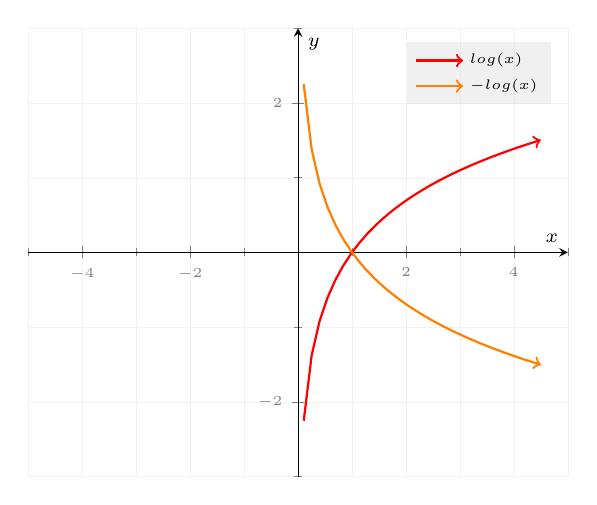
\begin{tikzpicture}
% axis settings {{{

\begin{axis}[
%	title          = graph_name,
	axis x line    = middle, % x-axis position
	axis y line    = middle, % y-axis position
	minor tick num = 1,      % num axis ticks
	grid           = both,
	grid style     =
	{
		line width = .1pt,
		draw       = gray!10
	},
	xmax      = 5,
	xmin      = -5,
	ymax      = 3,
	ymin      = -3,
	tick label style = {
		font  = \tiny,
		color = gray
	},
%	extra x ticks={3,1},
%	extra x tick labels={$\leftarrow$,$\rightarrow$},
%	extra y ticks={3,1},
%	extra y tick labels={$\leftarrow$,$\rightarrow$},
	legend style =
	{
		draw         = none, % remove legend bounding box
		font         = \tiny,
		legend pos   = north east,
		cells        = {anchor = west},
		fill         = gray!30,
		fill opacity = 0.4,
		text opacity = 1
	},
	xlabel       = {$\scriptstyle x$},
	ylabel       = {$\scriptstyle y$},
	xlabel style =
	{
		at     = {(ticklabel* cs:1)},
%		anchor = north west
	},
	ylabel style=
	{
		at     = {(ticklabel* cs:1)},
%		anchor = south west
	}
]
% }}}
\coordinate (O) at (0,0);

\addplot [
	domain=-10:4.5,
	samples=100,
	thick,
	red,
	->
]
{ln(x)};
\addlegendentry{$log(x)$};

\addplot [
	domain=-10:4.5,
	samples=100,
	thick,
	orange,
	->
]
{-ln(x)};
\addlegendentry{$-log(x)$};
\end{axis}
\end{tikzpicture}

% }}}
% ln(1-x)  {{{
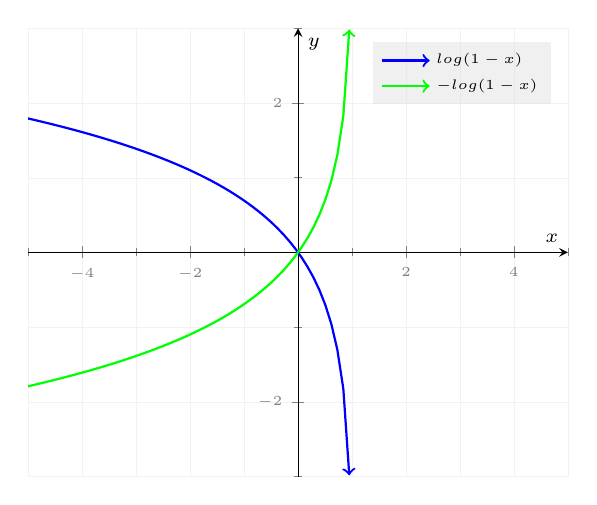
\begin{tikzpicture}
% axis settings {{{

\begin{axis}[
%	title          = graph_name,
	axis x line    = middle, % x-axis position
	axis y line    = middle, % y-axis position
	minor tick num = 1,      % num axis ticks
	grid           = both,
	grid style     =
	{
		line width = .1pt,
		draw       = gray!10
	},
	xmax      = 5,
	xmin      = -5,
	ymax      = 3,
	ymin      = -3,
	tick label style = {
		font  = \tiny,
		color = gray
	},
%	extra x ticks={3,1},
%	extra x tick labels={$\leftarrow$,$\rightarrow$},
%	extra y ticks={3,1},
%	extra y tick labels={$\leftarrow$,$\rightarrow$},
	legend style =
	{
		draw         = none, % remove legend bounding box
		font         = \tiny,
		legend pos   = north east,
		cells        = {anchor = west},
		fill         = gray!30,
		fill opacity = 0.4,
		text opacity = 1
	},
	xlabel       = {$\scriptstyle x$},
	ylabel       = {$\scriptstyle y$},
	xlabel style =
	{
		at     = {(ticklabel* cs:1)},
%		anchor = north west
	},
	ylabel style=
	{
		at     = {(ticklabel* cs:1)},
%		anchor = south west
	}
]
% }}}
\coordinate (O) at (0,0);

\addplot [
	domain=-10:0.95,
	samples=100,
	thick,
	blue,
	->
]
{ln(1-x)};
\addlegendentry{$log(1-x)$};

\addplot [
	domain=-10:0.95,
	samples=100,
	thick,
	green,
	->
]
{-ln(1-x)};
\addlegendentry{$-log(1-x)$};
\end{axis}
\end{tikzpicture}

% }}}
% ln(1-x)  {{{

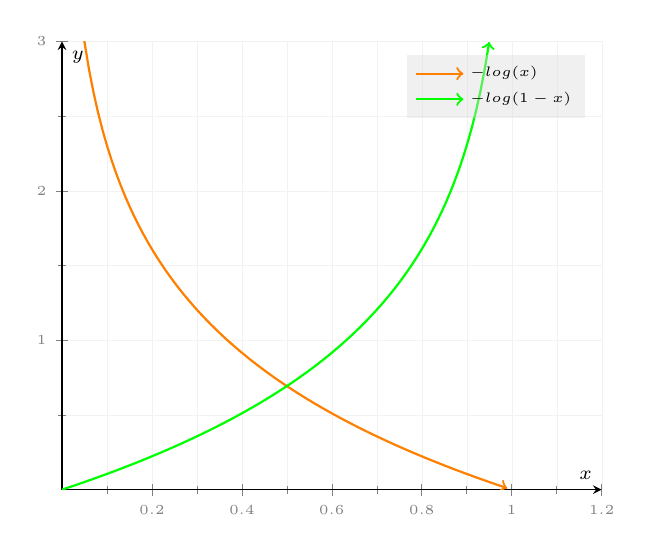
\begin{tikzpicture}
% axis settings {{{

\begin{axis}[
%	title          = graph_name,
	axis x line    = middle, % x-axis position
	axis y line    = middle, % y-axis position
	minor tick num = 1,      % num axis ticks
	grid           = both,
	grid style     =
	{
		line width = .1pt,
		draw       = gray!10
	},
	xmax      = 1.2,
	xmin      = 0,
	ymax      = 3,
	ymin      = 0,
	tick label style = {
		font  = \tiny,
		color = gray
	},
%	extra x ticks={3,1},
%	extra x tick labels={$\leftarrow$,$\rightarrow$},
%	extra y ticks={3,1},
%	extra y tick labels={$\leftarrow$,$\rightarrow$},
	legend style =
	{
		draw         = none, % remove legend bounding box
		font         = \tiny,
		legend pos   = north east,
		cells        = {anchor = west},
		fill         = gray!30,
		fill opacity = 0.4,
		text opacity = 1
	},
	xlabel       = {$\scriptstyle x$},
	ylabel       = {$\scriptstyle y$},
	xlabel style =
	{
		at     = {(ticklabel* cs:1)},
%		anchor = north west
	},
	ylabel style=
	{
		at     = {(ticklabel* cs:1)},
%		anchor = south west
	}
]
% }}}
\coordinate (O) at (0,0);

\addplot [
	domain=0:0.99,
	samples=100,
	thick,
	orange,
	->
]
{-ln(x)};
\addlegendentry{$-log(x)$};

\addplot [
	domain=0:0.95,
	samples=100,
	thick,
	green,
	->
]
{-ln(1-x)};
\addlegendentry{$-log(1-x)$};

\end{axis}
\end{tikzpicture}

% }}}

	Taking only the negative log from the graph and then using the interval
	only between $ 0 \leq x \leq 1$ , we get the following graph :

	Case y = 0
%	<img src="images/log_neg_interval.svg">
%	<img src="images/log_inv_neg_interval.svg">

\[
	\begin{array}{ l@{} l@{} l@{} } 
		\mathrm{Cost}(h_\theta(x),y)
		& = 0
		& \text{ if } h_\theta(x) = y 
		\\ 
		\mathrm{Cost}(h_\theta(x),y)
		& \rightarrow \infty
		&\text{ if } y = 0
		\; \mathrm{and} \;
		h_\theta(x) \rightarrow 1 
		\\ 
		\mathrm{Cost}(h_\theta(x),y)
		& \rightarrow \infty 
		& \text{ if } y = 1
		\; \mathrm{and} \;
		h_\theta(x) \rightarrow 0 
		\\ 
	\end{array}
\]

	\[
	\begin{array}{ l@{} l@{} } 
	J(\theta)
	& =
	\dfrac{1}{m}
	\sum_{i=1}^m
	\left\{
		\mathrm{Cost}(h_\theta(x^{(i)}),y^{(i)})
	\right\} 
	\\ 
	\mathrm{Cost}(h_\theta(x),y)
	& =
	\left\{ 
		\begin{array}{ l@{} l@{} } 
			-\log(h_\theta(x))
			\;
			& \text{if y = 1} 
			\\ 
			-\log(1-h_\theta(x))
			\;
			& \text{if y = 0} 
		\end{array}
	\right.  
	\\ 
	& = 
	-y\log(h_\theta(x))
	+
	(1-y)\log(1-h_\theta(x)) 
	\end{array}
\]


\[
	\begin{array}{ l@{} l@{} } 
	J(\theta)
	& =
	{ \displaystyle 
		\dfrac{1}{m}
		\sum_{i=1}^m
		\left\{
			\mathrm{Cost}(h_\theta(x^{(i)}),y^{(i)})
		\right\}
	}
	\\ 
	& =
	\dfrac{1}{m} 
	{ \displaystyle 
		\left(
			\sum_{i=1}^m
			\left\{
				-y^{(i)}\log(h_\theta(x^{(i)}))
				+
				(1-y^{(i)})\log(1-h_\theta(x^{(i)}))
			\right\}
		\right)
	} 
	\end{array}
\]

\subsectionend
% }}} END SUB-SECTION : cost_function
% 	SUB-SECTION : gradient_descent {{{
\subsection{Gradient Descent}
\label{ssec:gradient_descent}
\parindent=0em

	<h3>Logistic Regression : Gradient Descent</h3>

Just for reference cause we will need it later.

\[
	\begin{array}{ l@{} l@{} }
		\nabla J(\Theta)
		& =
		\left\langle
		  {\displaystyle \frac{\partial}{\partial \theta_0} J(\Theta)}
		, {\displaystyle \frac{\partial}{\partial \theta_1} J(\Theta)}
		, {\displaystyle \frac{\partial}{\partial \theta_2} J(\Theta)}
		\ldots
		, {\displaystyle \frac{\partial}{\partial \theta_m} J(\Theta)}
		\right\rangle
		\\
	\end{array}
\]


\[
	\begin{array}{ l@{} l@{} }
\sigma(x)             & = \frac{1}{1+e^{-x}} \\
\frac{d}{dx}\sigma(x) & = \frac{d}{dx} \left(  \frac{1}{1+e^{-x} } \right) \\
                      & = \frac{0 \cdot(1+e^{-x}) - (-e^{-x}) \cdot 1}{ ( 1+e^{-x} ) ^2} \text{$\hspace{46 mm}$Quotient rule}\\
                      & = \frac{e^{-x}}{ ( 1+e^{-x} ) ^2}  \\
                      & = \frac{(1+e^{-x}) -1 }{ ( 1+e^{-x} ) ^2} \\
                      & = \frac{ (1+e^{-x})}{ ( 1+e^{-x} ) ^2}  - \left( \frac{1}{1+e^{-x}} \right)^2\\
                      & = \frac{1}{1+e^{-x}}  - \left( \frac{1}{1+e^{-x}} \right)^2\\
                      & = \sigma (x) - \sigma(x)^2\\
\sigma^{'} (x)        & = \sigma(x)(1-\sigma(x))
	\end{array}
\]


We also have the following :
\[
	\begin{array}{ l@{} l@{} } 
		h_\theta(\Theta^T x)
		= \sigma(\Theta^Tx)
		& = \frac{1}{1+e^{-\Theta^T x}} \\ 
	\end{array}
\]

\[
\begin{array}{ l@{} l@{} l@{} l@{} } 
		P(y^{(i)} = 1 | x^{(i)} ; \theta)
		& = h_\theta(x)
		& = \sigma(x)
		& = \frac{1}{1+e^{-x}}
		\\ 
		P(y^{(i)} = 0 | x^{(i)} ; \theta)
		& = 1 - h_\theta(x)
		& = 1 - \sigma(x)
		& = 1 - \frac{1}{1+e^{-x}}
		\\ 
	\end{array}
\]

This gives us the overall likelihood of any outcome y given x and theta as :

\[
\begin{array}{ l@{} l@{} l@{} } 
		L(\theta) 
		& = P(y^{(i)}| x^{(i)} ; \theta)
		& = h(x^{(i)})^{y^{(i)}} \cdot ( 1 - h(x^{(i)}))^{1 - y^{(i)}} 
	\end{array}
\]

overall i's

\[
	\begin{array}{ l@{} l@{} }
	L(\theta) & =
	{ \displaystyle \prod_{i=1}^{m} }
	\left\{
		h
		\left(x^{(i)}\right)
		^{
			\left(
				y^{(i)}
			\right)
		}
		\cdot
		\left(
			1 - h(x^{(i)})
		\right)
		^{
			\left(
				1 - y^{(i)}
			\right)
		}
	\right\}
	\\
	\log(L(\theta)) & = \mathscr{L}(\theta) \\ 
	\mathscr{L}(\theta)
	& =
	\log \left( 
	{ \displaystyle \prod_{i=1}^{m} }
	\left\{
		h
		\left(x^{(i)}\right)
		^{
			\left(
				y^{(i)}
			\right)
		} 
		\cdot 
		\left(
			1 - h(x^{(i)})
		\right)
		^{
			\left(
				1 - y^{(i)}
			\right)
		} 
	\right\} 
	\right) 
	\\ 
	& = 
	{ \displaystyle \sum_{i=1}^{m} } \left\{ 
		\log \left( 
			h
			\left(x^{(i)}\right)
			^{
				\left(
					y^{(i)}
				\right)
			} 
			\cdot 
			\left(
				1 - h(x^{(i)})
			\right)
			^{
				\left(
					1 - y^{(i)}
				\right)
			} 
		\right) 
	\right\} 
	\\ 
	& = 
	{ \displaystyle \sum_{i=1}^{m} } \left\{ 
		\log \left( 
			h
			\left(x^{(i)}\right)
			^{
				\left(
					y^{(i)}
				\right)
			} 
		\right) 
		+ 
		\log \left( 
			\left(
				1 - h(x^{(i)})
			\right)
			^{
				\left(
					1 - y^{(i)}
				\right)
			} 
		\right) 
	\right\} 
	\\ 
	& = 
	{ \displaystyle \sum_{i=1}^{m} } \left\{ 
		\left(
			y^{(i)}
		\right) 
		\cdot 
		\log \left( 
		h \left(
			x^{(i)}
		\right) 
		\right) 
		+ 
		\left(
			1 - y^{(i)}
		\right) 
		\cdot 
		\log \left( 
		\left(
			1 -
			h \left(
				x^{(i)}
			\right) 
		\right) 
		\right) 
	\right\} 
	\end{array}
\]

We want to maximize the likelihood so we take the derivative :


\[
	\begin{array}{ l@{} l@{} r@{} } 
	{ \displaystyle \frac{\partial}{\partial \theta}}
	\mathscr{L}(\theta) 
	& = 
	{ \displaystyle \frac{\partial}{\partial \theta}}
	\left(
		{ \displaystyle \sum_{i=1}^{m} } \left\{ 
			\left(
				y^{(i)}
			\right) 
			\cdot 
			\log \left( 
			h \left(
				x^{(i)}
			\right) 
			\right) 
			+ 
			\left(
				1 - y^{(i)}
			\right) 
			\cdot 
			\log \left( 
			\left(
				1 -
				h \left(
					x^{(i)}
				\right) 
			\right) 
			\right) 
		\right\}
	\right) 
	\\ 
	& = 
	{ \displaystyle \frac{\partial}{\partial \theta}}
	\left(
		{ \displaystyle \sum_{i=1}^{m} } \left\{ 
			\left(
				y^{(i)}
			\right) 
			\cdot 
			\log \left( 
			\sigma \left(
				x^{(i)}
			\right) 
			\right) 
			+ 
			\left(
				1 - y^{(i)}
			\right) 
			\cdot 
			\log \left( 
			\left(
				1 -
				\sigma \left(
					x^{(i)}
				\right) 
			\right) 
			\right) 
		\right\}
	\right) 
	\\ 
	& = 
	{ \displaystyle \sum_{i=1}^{m} } \left\{ 
		\left(
			y^{(i)}
		\right) 
		\cdot 
		{ \displaystyle \frac{\partial}{\partial \theta}} \left( 
			\log \left( 
			\sigma \left(
				x^{(i)}
			\right) 
			\right) 
		\right) 
		+ 
		\left(
			1 - y^{(i)}
		\right) 
		\cdot 
		{ \displaystyle \frac{\partial}{\partial \theta}} \left( 
			\log \left( 
			\left(
				1 -
				\sigma \left(
					x^{(i)}
				\right) 
			\right) 
		\right) 
	\right\} 
	\right) 
	\\ 
	& = 
	{ \displaystyle \sum_{i=1}^{m} } \left\{ 
		\left(
			y^{(i)}
		\right) 
		\cdot 
		\left( 
			{ \displaystyle
			\frac
				{
					1
				}
				{
					\sigma \left( x^{(i)} \right)
				}
			} 
			\cdot 
			\sigma \prime \left( x^{(i)} \right) 
		\right) 
		+ 
		\left( 1 - y^{(i)} \right) 
		\cdot 
		\left( 
			{ \displaystyle
			\frac
				{
					1
				}
				{
					1 - \sigma \left( x^{(i)} \right)
				}
			} 
			\cdot 
			- \sigma \prime \left( x^{(i)} \right) 
		\right) 
	\right\} 
	& \text{Chain Rule} 
	\\ 
	& = 
	\end{array}
\]

Gradient Descent

\[
	\begin{array}{ l@{} l@{} } 
		\frac{\partial}{\partial \theta_0} J(\Theta)
		& =
		\left(
			\frac{1}{m}
			\cdot
			\sum_{i=1}^m \left\{
					\left(
						h_\theta(x^{(i)}) - y^{(i)}
					\right)^{2}
					\cdot
					x_{0}^{(i)}
			\right\}
		\right) 
		\\ 
		\frac{\partial}{\partial \theta_j} J(\Theta)
		& =
		\left(
			\frac{1}{m} \cdot
			\sum_{i=1}^m \left\{
				\left(
					h_\theta(x^{(i)}) - y^{(i)}
				\right)^{2}
				\cdot
				x_{j}^{(i)}
			\right\}
		\right) 
		+ 
		\frac{\lambda}{m}\cdot \theta_j 
		\\ 
	\end{array}
\]

The second sum, 
\( \frac{\lambda}{2m}
   \sum_{j = 1}^{n} {\theta_{j}^{2}} \)
means to explicitly exclude the bias term, $\theta_0$. i.e. the $\theta$
vector is indexed from 0 to n (holding n+1 values, $\theta_0$ through
$\theta_n$), and this sum explicitly skips $\theta_0$, by
running from 1 to n, skipping 0. Thus, when computing the equation, we should
continuously update the two following equations:

	\[
	\begin{array}{ l@{} l@{} l@{} l@{} } 
		\theta_0
		& := &
		\theta_0
		- \alpha
		\cdot
		\left(
		\frac{1}{m}
		\cdot 
			\sum_{i=1}^m
			\left\{
				\left(
					h_\theta(x^{(i)}) - y^{(i)}
				\right)^{2}
				\cdot
				x_{0}^{(i)}
			\right\}
		\right) 
		\hspace{0.5cm} & \text{for} \; j = 0 
		\\ 
		\theta_j
		& := &
		\theta_j
		- \alpha
		\cdot
		\left(
		\frac{1}{m}
		\cdot 
			\sum_{i=1}^m
			\left\{
				\left(
					h_\theta(x^{(i)}) - y^{(i)}
				\right)^{2}
				\cdot
				x_{j}^{(i)}
				+
				\left(
					\frac{\lambda}{m}\cdot \theta_j
				\right)
			\right\}
		\right) 
		\hspace{0.5cm} & \text{for} \; j = 1,2, \ldots , n 
		\\ 
		& :=
		& \theta_j
		\cdot
		(1 - \alpha \cdot \frac{\lambda}{m})
		-
		\alpha
		\cdot
		\left(
		\frac{1}{m}
		\cdot 
			\sum_{i=1}^m
			\left\{
				\left(
					h_\theta(x^{(i)}) - y^{(i)}
				\right)^{2}
				\cdot
				x_{j}^{(i)} 
			\right\}
		\right) 
		\\ 
		\end{array}
	\]
\subsectionend
% }}} END SUB-SECTION : gradient_descent
% 	SUB-SECTION : extra {{{
\subsection{Extra}
\label{ssec:extra}
\parindent=0em

% 		SUB-SUB-SECTION : advanced_optimization_algorithms {{{
\subsubsection{Advanced Optimization Algorithms}
\label{sssec:advanced_optimization_algorithms}
\parindent=0em


	<h3>Advanced Optimization Algorithms</h3>

	The various advanced optimization algorithms are :


	<ul>
		<li>Gradient Descent</li>
		<li>Conjugate gradient</li>
		<li>BFGS</li>
		<li>L-BFGS</li>
	</ul>

\subsubsectionend
% }}} END SUB-SUB-SECTION : advanced_optimization_algorithms
% 		SUB-SUB-SECTION : multiclass_classification {{{
\subsubsection{Multiclass Classification}
\label{sssec:multiclass_classification}
\parindent=0em

	<h3>Logistic Regression : Multiclass Classification</h3>

	<p>

		To do multiclass classification , we use a method called one-vs-all (
		sometimes also called one-vs-rest ). In this method we will train a new
		classfier with a spereate hypothesis function $h_\theta(x)$ for each
		thing we want to classify.  So if we want to classify k different things
		, we will have k different hypothesis functions. These will be denoted
		using a superscript $h_\theta^{(k)}(x)$.
		
		
		\[
			\begin{array}{ l@{} l@{} }
				h_\theta^{(i)}(x) = P(y=i|x;\theta) \; , \; 1 \leq i \leq k , k
				\in \mathbb{N}
			\end{array}
		\]


		The probability equation is telling us what the probability is that the
		x value we are looking at belongs in the current class k. <br> <br>

		What this means is that for each class k , when we recieve a new data
		point we dont have to decide which specific class it belongs into yet.
		All we have to do is figure out if it belongs in the current class that
		we are looking at. So does it belong in the current class or one of all
		of the rest of the classes , doesnt matter which. Then we repeat this
		process until we figure out which one it belongs to , by iterative
		comparison of one-vs-all.  <br> <br>

		So at the end we just pick the hypothesis that maximizes the probability
		that a given item x belongs in class k : 
		
		\[
			\begin{array}{ l@{} l@{} }
				\max\limits_i h_\theta^{(i)}(x) &
			\end{array}
		\]

	</p>


\subsubsectionend
% }}} END SUB-SUB-SECTION : multiclass_classification
% 		SUB-SUB-SECTION : overfitting {{{
\subsubsection{Overfitting}
\label{sssec:overfitting}
\parindent=0em

	<h3>Overfitting</h3>

	If we have too many features , the learned hypothesis may fit the training
	set very well , i.e. , 

	\[
		\begin{array}{ l@{} l@{} }


			J(\theta)
			= \frac{1}{2m}
			\sum_{i=1}^m
			\left\{
				\left(
					h_\theta(x^{(i)}) - y^{(i)}
				\right)^{2}
			\right\}

			\approx 0


		\end{array}
	\]

	but this function may fail to generalize to new examples.<br> <br>

	<b> Underfitting </b>, or <b> high bias </b>, is when the form of our
	hypothesis function h maps poorly to the trend of the data. It is usually
	caused by a function that is too simple or uses too few features.<br> <br>

	At the other extreme, <b> overfitting </b>, or <b> high variance </b>, is
	caused by a hypothesis function that fits the available data but does not
	generalize well to predict new data. It is usually caused by a complicated
	function that creates a lot of unnecessary curves and angles unrelated to
	the data.<br> <br>

	There are a couple of things we can do to reduce over fitting :


	<ol>
		<li>Reduce number of features</li>
		<ol>
			<li>Manually select which features to keep</li>
			<li>Use a model selection algorithm</li>
		</ol>
		<li>Use Regularization</li>
		<ol>
			<li>Keep all the features , but reduce the magnitude / values of the
				parameters $\theta_j$ </li>
			<li>Works well when we have a lot of features , each one of whic
				contribute a little bit towards predictin $y$</li>
		</ol>
	</ol>


\subsubsectionend
% }}} END SUB-SUB-SECTION : overfitting
% 		SUB-SUB-SECTION : regularization {{{
\subsubsection{Regularization}
\label{sssec:regularization}
\parindent=0em

<h3>Regularization</h3>

To fix the problem of overfitting one of the things that we prefer is for the
hypothesis to be as simple as possible. This means that we want to reduce the
effect ( as close to zero as we can ) of the higher order polynomials as we can.
In order to do this we can introduce a regularization term. The purpose of this
term is to penalize the cost function (by assigning a higher value) when it
assigns higher weight ( larger values for $\theta_j$ ) to higher order
polynomials. This means the higher the order of the $x$ value the more the cost
function will be rewarded if it DOES NOT include it as a significant contibutor.
Keep in mind we are using the same amount of features $x_(j)^{(i)}$ , all we are
doing is reducing the polynomial order of the features. The cost function is not
being penalized for reducing the impact of the features theselves.<br>

The regularization term looks like :

\[
	\begin{array}{ l@{} l@{} } 
		\frac{1}{2} \cdot
		\frac{1}{m} \cdot 
		\lambda \cdot
		\sum_{j = 1}^{n}
		\left\{
			{\theta_{j}^{2}}
		\right\} 
	\end{array}
\]

$\lambda$ is called the regularization parameter. Its job is to control the
tradeoff between two different goals. The first goal is to actually fit the
training data well. This is done by our original cost function $J(\theta)$. The
second goal is to keep the parameters small. This makes our Cost function now
look like :

\[
	\begin{array}{ l@{} l@{} } 
		J(\theta)
		=
		\left( 
		\frac{1}{2}
		\cdot
		\frac{1}{m}
		\cdot 
			\left(
				\sum_{i=1}^m
				\left\{
					\left(
						h_\theta(x^{(i)}) - y^{(i)}
					\right)^{2}
				\right\}
			\right) 
			+
			\left( 
				\frac{1}{2} \cdot
				\frac{1}{m} \cdot 
				\lambda \cdot
				\sum_{j = 1}^{n}
				\left\{
					{\theta_{j}^{2}}
				\right\}
			\right)
		\right) 
	\end{array} 
\]


Keep in mind though that if we set \( lambda \) to be some huge value like


\( \lambda = 10^{10} \) then we might not even achieve our primary objective of
fitting the data well since we are punishing the cost function too much. This
would basically mean that each \( \theta_j \approx 0 \; , \; j \geq 1 \) and we
would effectively only be left with \( h_{\theta}(x) = \theta_0 \) which is
basically just a straight line through the intercept.  This would result in a
case of underfitting due to a too large \( \lambda \) value.

	<h3>Regularized Linear Regression</h3>

	\[
		\begin{array}{ l@{} l@{} } 
			\min\limits_\theta
			J(\theta)
			=
			\frac{1}{2}
			\cdot
			\frac{1}{m}
			\cdot
			\left(
				\left(
					\sum_{i=1}^m
					\left\{
						\left(
							h_\theta(x^{(i)}) - y^{(i)}
						\right)^{2}
					\right\}
				\right) 
				+
				\left( 
					\frac{1}{2} \cdot
					\frac{1}{m} \cdot
					\lambda \cdot
					\sum_{j = 1}^{n}
					\left\{
						{\theta_{j}^{2}}
					\right\}
				\right)
			\right) 
		\end{array} 
	\]


\subsubsectionend
% }}} END SUB-SUB-SECTION : regularization

\subsectionend
% }}} END SUB-SECTION : extra

%	{{{
<h3>Logistic Regression</h3>

This is a type of classification algorithm , as opposed to linear or non-linear
regression algorithms which all relied on predicting continuous values , a
classifcation algirthm will use the independent variables (features) to predict
binary values like : Yes / No , True / False , Malignant / Non-Malignant ,
Pregnant / Not-Pregnant etc... All these examples are binary beacuse that is
what I am going to be using in this explanation , but we can use multiple
logistic regression with vectors to extend the algorithm for multi-class
classification to classify the output into as many fields as we like.<br>

Even though the dependant variables are discrete classifications , the
independant variables $x_j$ values should all be continous.<br>

Logistic Regression measures the probability of a case belonging to a specific
class. Logistic Regression can be used to understand the impact of a feature on
a dependant variable. <br>

<ul>

	<li>Input / independant Variables : $ X \in \mathbb{R}^{m \times n}$</li>
	<li>Output / dependant Variables : $ y \in \{0,1\}$</li>
	<li>: $ \hat{y} = P(y=1|x) $</li>
	<li>: $ P(y=0|x) = 1 - P(y=1|x) $</li>
</ul>

We can use the equations we have from linear regression as outr starting poing
for logistic regression. We have :

			\[
				\begin{array}{ l@{} l@{}} 
				\Theta_{(n \times 1)} = 
				\begin{bmatrix} 
				\theta_0 \\
				\theta_1 \\
				\theta_2 \\
				\vdots \\
				\theta_n \\ 
				\end{bmatrix} 
				\; , \; 
				\Theta_{(1 \times n)}^{T} = 
				\begin{bmatrix} 
				\theta_0 ,
				\theta_1 ,
				\theta_2 ,
				\cdots , 
				\theta_n
				\end{bmatrix} 
				\; , \; 
				X_{(n \times 1)} = 
				\begin{bmatrix} 
					1 \\
					x_1 \\
					x_2 \\
					\vdots \\
					x_n \\ 
				\end{bmatrix} \\ 
				\end{array}
			\]

			\[
			\begin{array}{ l@{} l@{} l@{} l@{} } 
			\hat{y}
			& = h_\theta (x)
			& = \Theta_{(1 \times n)}^{T} \cdot X_{(n \times 1)} 
			& = 
			\begin{bmatrix} 
				\theta_0 \\
				\theta_1 \\
				\theta_2 \\
				\vdots \\
				\theta_n \\ 
			\end{bmatrix}_{(1 \times n)} 
			\cdot 
			\begin{bmatrix} 
				1 \\
				x_1 \\
				x_2 \\
				\vdots \\
				x_n \\ 
			\end{bmatrix}_{(n \times 1)} 
			\\ 
			& & & =
			\begin{bmatrix} 
				x_0\theta_0 +
				x_1\theta_1 +
				x_2\theta_2 +
				\cdots +
				x_n\theta_n \\ 
			\end{bmatrix}_{(1 \times 1)} 
			\end{array}
			\] 

\[
	\begin{array}{ l@{} l@{} l@{}} 
		\Theta^T X & = & \theta_0 x_0 + \theta_1 x_1 + \theta_2 x_2 + \ldots +
		\theta_n x_n \\
		h_\theta (x) & = & \Theta^T X \\ 
	\end{array}
\]

<h4>The Training Process</h4>

<ol>
	<li>Initialize $\theta$</li>
	<li>Calculate $ \hat{y} = \sigma(\Theta^{T} X)$</li>
	<li>Compare the output of $\hat{y}$ with actual output of cutomer , y, and
		record it as error.</li>
	\[
		\begin{array}{ l@{} l@{} } 
			Error = 1 - 
			\left(
				\hat{y} = \sigma(\theta^{T} X)
			\right)
		\end{array}
	\]
	<li>Calcualte error for all customers $Cost = J(\theta)$</li>
	<li>Change $\theta$ to reduce the cost</li>
	<li>Go back to step 2</li>
</ol>

\[
	\begin{array}{ l@{} l@{} } 
	\widehat{y} = \sigma(\theta_1 x_1 + \ldots + \theta_n x_n) 
	\end{array}
\]

\[
	\begin{array}{ l@{} l@{} } 
		J(\theta)
		& =
		-
		\frac{1}{m}
		\cdot
		\sum_{i=1}^{m}
		\left\{
			y^{i}
			log(\widehat{y^{i}})
			+
			(1 - y^{i})
			log(1-\widehat{y^{i}})
		\right\}
	\end{array}
\]

\[
	\begin{array}{ l@{} l@{} } 
		\frac{\partial}{\partial \theta_0} J(\theta_1)
		& =
		-
		\frac{1}{m}
		\cdot 
		\sum_{i=1}^m
		\left\{
			\left(
				y^{i} - \widehat{y^{i}}
			\right)
			\cdot
			x_{1}^{i}
		\right\} 
	\end{array}
\]

Using gradient descent the gradient vector is :

\[
	\begin{array}{ l@{} l@{} } 
		\nabla J
		& = 
		\begin{bmatrix} 
			\frac{\partial J(\theta_1)}{\partial \theta_1}  \\ 
			\frac{\partial J(\theta_2)}{\partial \theta_2}  \\ 
			\vdots \\ 
			\frac{\partial J(\theta_k)}{\partial \theta_k}  \\ 
		\end{bmatrix} 
	\end{array}
\]

update equation :

\[
	\begin{array}{ l@{} l@{} } 
	\theta_{new} = \theta_{prev} - \eta \nabla J 
	\end{array}
\]


%	  }}}


%\sectionend
% }}} END SECTION : logistic_regression
